% De FT a espacio de estados — forma canónica controlable (2.º orden)
% G(s) = (b1 s + b0)/(s^2 + a1 s + a0)
\documentclass[border=6pt]{standalone}
\usepackage{amsmath}
\usepackage{tikz}
\usetikzlibrary{arrows.meta, calc}
\begin{document}
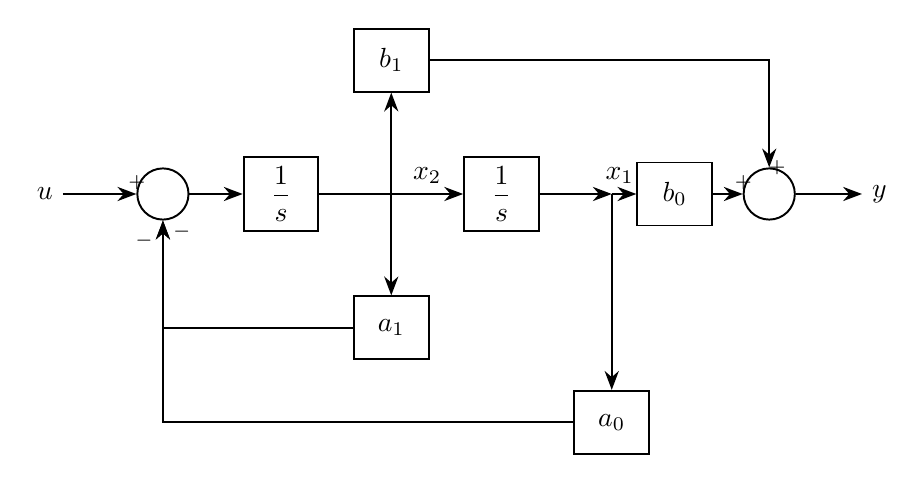
\begin{tikzpicture}[
  >={Stealth[length=2.4mm]}, line width=0.7pt,
  block/.style={draw, minimum width=0.95cm, minimum height=0.8cm},
  sum/.style={draw, circle, minimum size=6.5mm, inner sep=0pt}]

  % cadena de integradores
  \node (u)  at (0,0)        {$u$};
  \node[sum]   (S)  at (1.5,0)  {};
  \node[block] (I2) at (3.0,0)  {$\dfrac1s$};
  \coordinate (x2) at (4.4,0);
  \node[block] (I1) at (5.8,0)  {$\dfrac1s$};
  \coordinate (x1) at (7.2,0);

  \draw[->] (u) -- (S);
  \draw[->] (S) -- (I2);
  \draw[-]  (I2) -- (x2);
  \draw[->] (x2) -- (I1) node[midway, above]{$x_2$};
  \draw[->] (I1) -- (x1);
  \node[above] at ($(x1)+(0.1,0)$) {$x_1$};

  % salida: y = b0 x1 + b1 x2
  \node[sum]   (Sy) at (9.2,0) {};
  \node (y)    at (10.6,0) {$y$};
  \node[block] (b0) at (8.0,0) {$b_0$};
  \draw[->] (x1) -- (b0);
  \draw[->] (b0) -- (Sy);
  \draw[->] (Sy) -- (y);
  \node[block] (b1) at (4.4,1.7) {$b_1$};
  \draw[->] (x2) -- (b1);
  \draw[->] (b1) -| (Sy);
  \node at ($(Sy)+(-0.33,0.15)$) {\scriptsize$+$};
  \node at ($(Sy)+(0.1,0.33)$) {\scriptsize$+$};

  % realimentación: -a1 x2,  -a0 x1
  \node[block] (a1) at (4.4,-1.7) {$a_1$};
  \draw[->] (x2) -- (a1);
  \draw[->] (a1) -| (S) node[pos=0.95, right]{\scriptsize$-$};
  \node[block] (a0) at (7.2,-2.9) {$a_0$};
  \draw[->] (x1) -- (a0);
  \draw[->] (a0) -| (S) node[pos=0.95, left]{\scriptsize$-$};
  \node at ($(S)+(-0.33,0.15)$) {\scriptsize$+$};
\end{tikzpicture}
\end{document}
